\begin{figure}[!ht]
\centering
\begin{subfigure}[c]{0.525\textwidth}
\centering
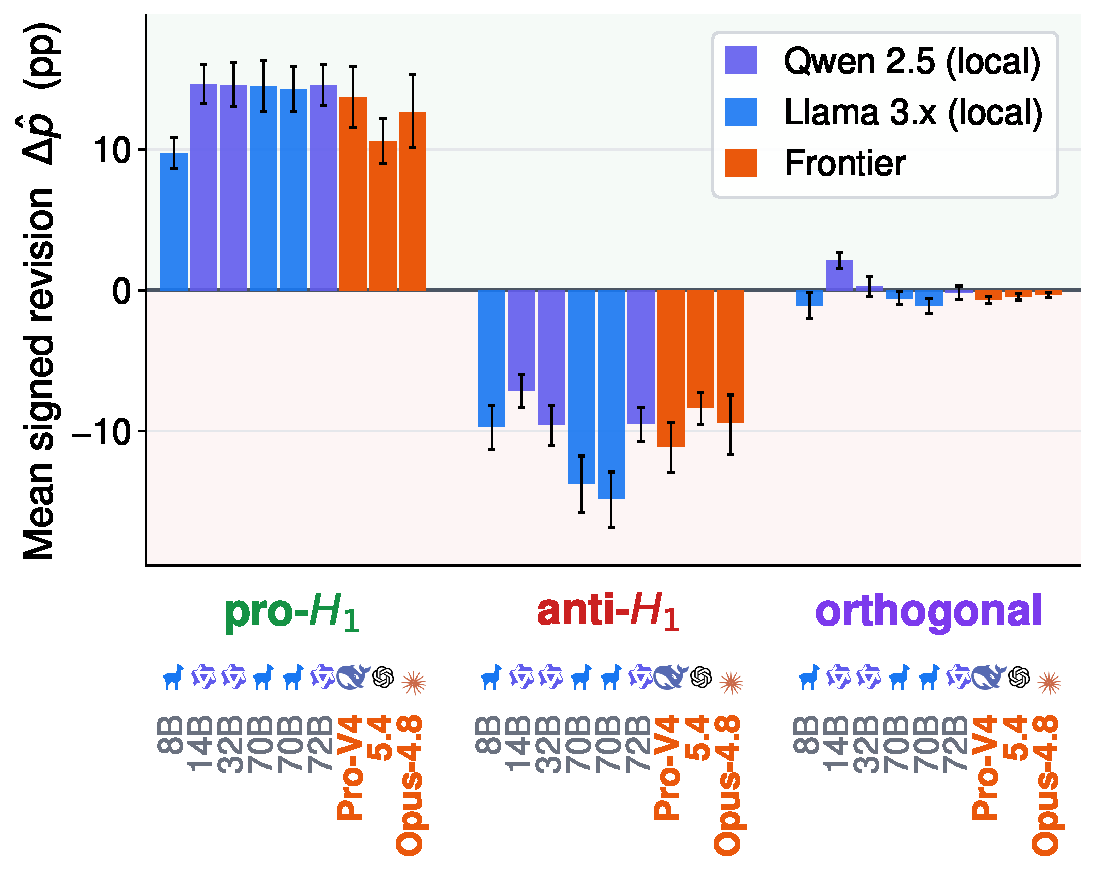
\includegraphics[width=\linewidth]{figures/exp1_direction_selective_updating.pdf}
\caption{}
\label{fig:exp1-bars}
\end{subfigure}\hspace{0.01\textwidth}
\begin{subfigure}[c]{0.455\textwidth}
\centering
\footnotesize
\setlength{\tabcolsep}{3pt}
\begin{tabular*}{\linewidth}{@{}l@{\extracolsep{\fill}}rccc@{}}
\toprule
\textbf{Model} & \textbf{Size} & \textbf{Abst.} & \textbf{Sens.}$\uparrow$ & \textbf{EHC$_{\geq3}$}$\uparrow$ \\
\midrule
\multicolumn{5}{@{}l}{\emph{Hosted API (parameters undisclosed)}}\\
\micon{claude.png}~Opus~4.8 & --- & 71.4\% & \cellcolor{heatgreen}$7.0\times$ & \cellcolor{heatgreen}.990 \\
\micon{openai.png}~GPT-5.4 & --- & 8.4\% & \cellcolor{heatgreen}$7.5\times$ & \cellcolor{heatgreen}.987 \\
\micon{deepseek.png}~V4-Pro & --- & 44.4\% & \cellcolor{heatyellow}$4.9\times$ & \cellcolor{heatyellow}.977 \\
\midrule
\multicolumn{5}{@{}l}{\emph{Open-weight, descending parameters} $\downarrow$}\\
\micon{qwen.pdf}~2.5-72B & 72B & 24.2\% & \cellcolor{heatorange}$3.2\times$ & \cellcolor{heatyellow}.963 \\
\micon{llamma.pdf}~3.3-70B & 70B & 10.7\% & \cellcolor{heatyellow}$5.7\times$ & \cellcolor{heatyellow}.965 \\
\micon{llamma.pdf}~3.1-70B & 70B & 2.5\% & \cellcolor{heatyellow}$4.5\times$ & \cellcolor{heatyellow}.961 \\
\micon{qwen.pdf}~2.5-32B & 32B & 11.1\% & \cellcolor{heatorange}$2.8\times$ & \cellcolor{heatyellow}.964 \\
\micon{qwen.pdf}~2.5-14B & 14B & 26.1\% & \cellcolor{heatred}$2.2\times$ & \cellcolor{heatorange}.943 \\
\micon{llamma.pdf}~3.1-8B & 8B & 1.1\% & \cellcolor{heatred}$1.9\times$ & \cellcolor{heatred}.887 \\
\bottomrule
\end{tabular*}
\caption{}
\label{fig:exp1-table}
\label{tab:consistency}
\end{subfigure}
\caption{\textbf{Direction-selective updating across nine models and 30,094 valid update
records.} \textbf{(a)} Mean signed forecast revision by counterfactual direction;
error bars are 95\% market-clustered bootstrap intervals. The orthogonal arm
carries no intended sign, so its signed mean is near zero by construction; its
absolute revisions are $0.5$--$5.9$~pp. \textbf{(b)} Hosted systems first,
open-weight rows in descending parameter count; measures and color bands are
defined in Methods, and abstention is uncolored because a high rate is not
unambiguously better. Appendix Table~\ref{tab:exp1-abstention} gives the product
of the two selectivity measures, and
Appendix~\ref{app:exp1-threshold-robustness} the output-field compliance and
threshold sweep.}
\label{fig:exp1-updating}
\end{figure}

\subsection{Experiment 1: Evidence-Selective Forecast Updating}
\label{sec:exp1}

Experiment~1 asks whether forecasts respond to probative evidence more than to
topic-matched controls. The agent sees only its own prior forecast and the
snippet: no packet names $H_1$, $H_2$, or the market's resolution, and 2.4\% use
any likelihood wording at all (Appendix~\ref{app:exp1-withholding}). The direction
key is therefore never supplied, although the snippet's words can carry partial
directional signal.

\textbf{Discrimination.} Selective updating has two separable components, and the
table reports them side by side. The first is declining to revise at all: every
deployment holds the prior on $1.1$--$71.4\%$ of topic-matched controls but on
only $0.0$--$1.4\%$ of directional packets. The second is how far it moves when it
does move, which is $1.9$--$7.5\times$ farther on directional packets, every
market-clustered 95\% interval excluding one. A ratio can be inflated by a small
denominator, so two checks avoid dividing: every model moves further on
directional packets in every market it covers, and the within-market probability
that it does so for a random packet pair runs from $.791$ to $.994$. Hosted
systems lead on both components on average, but neither separates the two classes
(Appendix~\ref{app:exp1-alternatives}).

\textbf{Directional correctness.} Across 30,094 valid updates, EHC runs from .887
to .990. All three hosted agents exceed .97; without the three-point movement
threshold, their correctness remains 97.3--98.4\%. A bag-of-words classifier trained on the packet
texts, markets held out, recovers the sign at $.688$, and adding the market
question does not help. Eight human reviewers match the frozen direction on
75.0\% of judgments in a smaller, categorical materials check (pairwise
$\kappa=.47$; Appendix~\ref{app:exp1-human-review}). The tasks are not a
human--model ranking. They show that wording carries partial signal, but this
shallow classifier falls well short of the agents' $.89$--$.99$ directional
accuracy. This within-directional-arm comparison does not depend on the
orthogonal arm's different wording.

Two caveats qualify the selectivity result. Wording differs across arms, so models
may use arm-correlated cues rather than derive relevance, although stated relevance
predicts their updates (Appendix~\ref{app:exp1-alternatives}). The tested
relationships may also be familiar; Experiment~2 requires inferring a novel one.
Full protocol, robustness, and materials details appear in
Appendix~\ref{app:exp1}.
